\let\negmedspace\undefined
\let\negthickspace\undefined
\documentclass[journal]{IEEEtran}
\usepackage[a5paper, margin=10mm, onecolumn]{geometry}
%\usepackage{lmodern} % Ensure lmodern is loaded for pdflatex
\usepackage{tfrupee} % Include tfrupee package

\setlength{\headheight}{1cm} % Set the height of the header box
\setlength{\headsep}{0mm}     % Set the distance between the header box and the top of the text

\usepackage{gvv-book}
\usepackage{gvv}
\usepackage{cite}
\usepackage{amsmath,amssymb,amsfonts,amsthm}
\usepackage{algorithmic}
\usepackage{graphicx}
\usepackage{textcomp}
\usepackage{xcolor}
\usepackage{txfonts}
\usepackage{listings}
\usepackage{enumitem}
\usepackage{mathtools}
\usepackage{gensymb}
\usepackage{comment}
\usepackage[breaklinks=true]{hyperref}
\usepackage{tkz-euclide} 
\usepackage{listings}
% \usepackage{gvv}                                        
\def\inputGnumericTable{}                                 
\usepackage[latin1]{inputenc}                                
\usepackage{color}                                            
\usepackage{array}                                            
\usepackage{longtable}                                       
\usepackage{calc}                                             
\usepackage{multirow}                                         
\usepackage{hhline}                                           
\usepackage{ifthen}
\usepackage{lscape}
\begin{document}

\bibliographystyle{IEEEtran}

\title{2.10.85}
\author{EE25BTECH11057 - Rushil Shanmukha Srinivas
}
% \maketitle
% \newpage
% \bigskip
{\let\newpage\relax\maketitle}

\renewcommand{\thefigure}{\theenumi}
\renewcommand{\thetable}{\theenumi}
\setlength{\intextsep}{10pt} % Space between text and floats

\numberwithin{equation}{enumi}
\numberwithin{figure}{enumi}
\renewcommand{\thetable}{\theenumi}



\textbf{Problem:} Let P be the plane 3x+2y+3z=16 and let S: $\alpha\hat{i} + \beta\hat{j} + \gamma\hat{k} $ ,where $\alpha+\beta+\gamma=7$ and the distance of $(\alpha,\beta,\gamma)$ from the plane is $2/{\sqrt{22}}$ .Let $\vec{u},\vec{v},\vec{w}$ be three distinct vectors in S such that $|\vec{u}-\vec{v}|=|\vec{v}-\vec{w}|=|\vec{w}-\vec{u}|$. Let V be the volume of the parallelopiped determined by vectors $\vec{u},\vec{v},\vec{w}$. Then the value of (80/3)V is 

\textbf{Solution:}

\begin{align}
P:\; \vec{n}^\top \vec{x} = c,\qquad \vec{n}=\myvec {3\\2\\3}\;c=16, \vec{O}=\myvec{0\\0\\0}
\end{align}

The distance of point $\vec{P_0}=\myvec{\alpha\\ \beta\\ \gamma}$ from the plane is
\begin{align}
\operatorname{dist}(\vec{P_0},P)=\frac{|\vec{n}^\top \vec{P_0} - c|}{\norm{\vec{n}}}
\end{align}
Given $\alpha+\beta+\gamma=7$ and $\operatorname{dist}(\vec{P_0},P)=\tfrac{2}{\sqrt{22}}$, we have
\begin{align}
\frac{|3\alpha+2\beta+3\gamma-16|}{\sqrt{22}}=\frac{2}{\sqrt{22}}
\;\;\Longrightarrow\;\; \vec{n}^\top \vec{P_0}=18 \;\;\text{or}\;\; \vec{n}^\top \vec{P_0}=14.
\end{align}

Thus $S$ lies on the intersections
\begin{align}
\Pi:\; \vec{m}^\top \vec{x}=7,\qquad \vec{m}=\myvec{1\\1\\1},
\end{align}
with
\begin{align}
P_+: \vec{n}^\top \vec{x}=18,\qquad P_-:\vec{n}^\top \vec{x}=14.
\end{align}

\textbf{(i) Intersection of $\vec{m}^\top \vec{x}=7$ and $\vec{n}^\top \vec{x}=18$.}\\
Write the augmented system in matrix form:
\begin{align}
\myvec
{1 & 1 & 1 &\vrule& 7\\[4pt]
3 & 2 & 3 &\vrule& 18} \xrightarrow{R_2 \longrightarrow R_2-3R_1}
\myvec{
1 & 1 & 1 &\vrule& 7\\[4pt]
0 & -1 & 0 &\vrule& -3}.
\end{align}
From the second row we get  $y=3$. Substitute into $x+y+z=7$:
\begin{align}
x+3+z=7 \quad\Longrightarrow\quad z=4-x.
\end{align}
So the line is
\begin{align}
\vec{L_1} = \myvec{0\\3\\4} + k_1\myvec{1\\0\\-1} = \vec{a} + k_1 \vec{d} 
\end{align}

\textbf{(ii) Intersection of $\vec{m}^\top \vec{x}=7$ and $\vec{n}^\top \vec{x}=14$.}\\
The augmented matrix is
\begin{align}
\myvec
{1 & 1 & 1 &\vrule& 7\\[4pt]
3 & 2 & 3 &\vrule& 14} \xrightarrow{R_2 \longrightarrow R_2-3R_1}
\myvec
{1 & 1 & 1 &\vrule& 7\\[4pt]
0 & -1 & 0 &\vrule& -7}.
\end{align}
So  $y=7$. From $x+y+z=7$ we get
\begin{align}
x+7+z=7 \quad\Longrightarrow\quad z=-x.
\end{align}
\begin{align}
\vec{L_2} = \myvec{0\\7\\0} + k_2\myvec{1\\0\\-1} = \vec{b} + k_2 \vec{d}
\end{align}
 hence the two lines are parallel.
 
 \textbf{(iii) Perpendicular distance between the two parallel lines}:
 $\vec{P}=\vec{a}+p_1 \vec{d} \ and\ \vec{Q}=\vec{b}+p_2 \vec{d} \ be \ 2 points\ on\ \vec{L_1},\vec{L_2}. $
\begin{align} 
perpendicular\ distance = \operatorname{dist}(\vec{P},\vec{Q}) ,\vec{M}=\myvec{\vec{d} & \vec{d}} 
\end{align}
 \begin{align}
 \vec{M}^\top(a-b) + \vec{M}^\top\vec{M}\myvec{p_1\\-p_2} = 0 , 
 \end{align}
 \begin{align}
 \myvec{\vec{d}\\\vec{d}}(a-b) + \myvec{\vec{d}\\\vec{d}}\myvec{\vec{d} & \vec{d}}\myvec{p_1\\-p_2} = 0
 \end{align}
On solving we get , 
\begin{align}
p_1 - p_2 = 2 \ take \ p_1=2 \ and \ p_2=0
\end{align}
 Points are $\vec{P}=\myvec{2\\3\\2} , \vec{Q}=\myvec{0\\7\\0},\vec{P}-\vec{Q}=\myvec{2\\-4\\2}$
 \begin{align}
Distance = D= {\norm{\vec{P}-\vec{Q}}} = \sqrt{24} 
\end{align}
\textbf{(iv) Area of the equilateral triangle formed by $\vec{u},\vec{v},\vec{w}$}:
As the two lines are parallel and let s = length of side of triangle
\begin{align}
D = \frac{\sqrt{3}s}{2} \Longrightarrow s = 4\sqrt{2}
\end{align}
\begin{align}
\text Area \ of\ the\ equilateral\ triangle = A = \frac{\sqrt{3}s^2}{4} = 8\sqrt{3} 
\end{align}
\textbf{(v) Volume of the parallelepiped determined by three vectors $\vec{u},\vec{v},\vec{w}$}:
$Volume\ of\ Parallelepiped = 6(Volume\ of\ Tetrahedron) = 2\times base\ area\times height$
Height=h=Perpendicular distance from origin to plane containing $\vec{u},\vec{v},\vec{w}$  
\begin{align}
h=\frac{|\vec{m}^\top\vec{O}-c|}{\norm{\vec{m}}}=\frac{|0-7|}{\sqrt{3}}=\frac{7}{\sqrt{3}}
\end{align}
\begin{align}
Volume = 2\times8\sqrt{3}\times\frac{7}{\sqrt{3}} = 112
\end{align}

\begin{align}
\frac{80}{3}V = \frac{80}{3}\times 112 = \frac{8960}{3}.
\end{align}




\begin{figure}[h!]
  \centering
  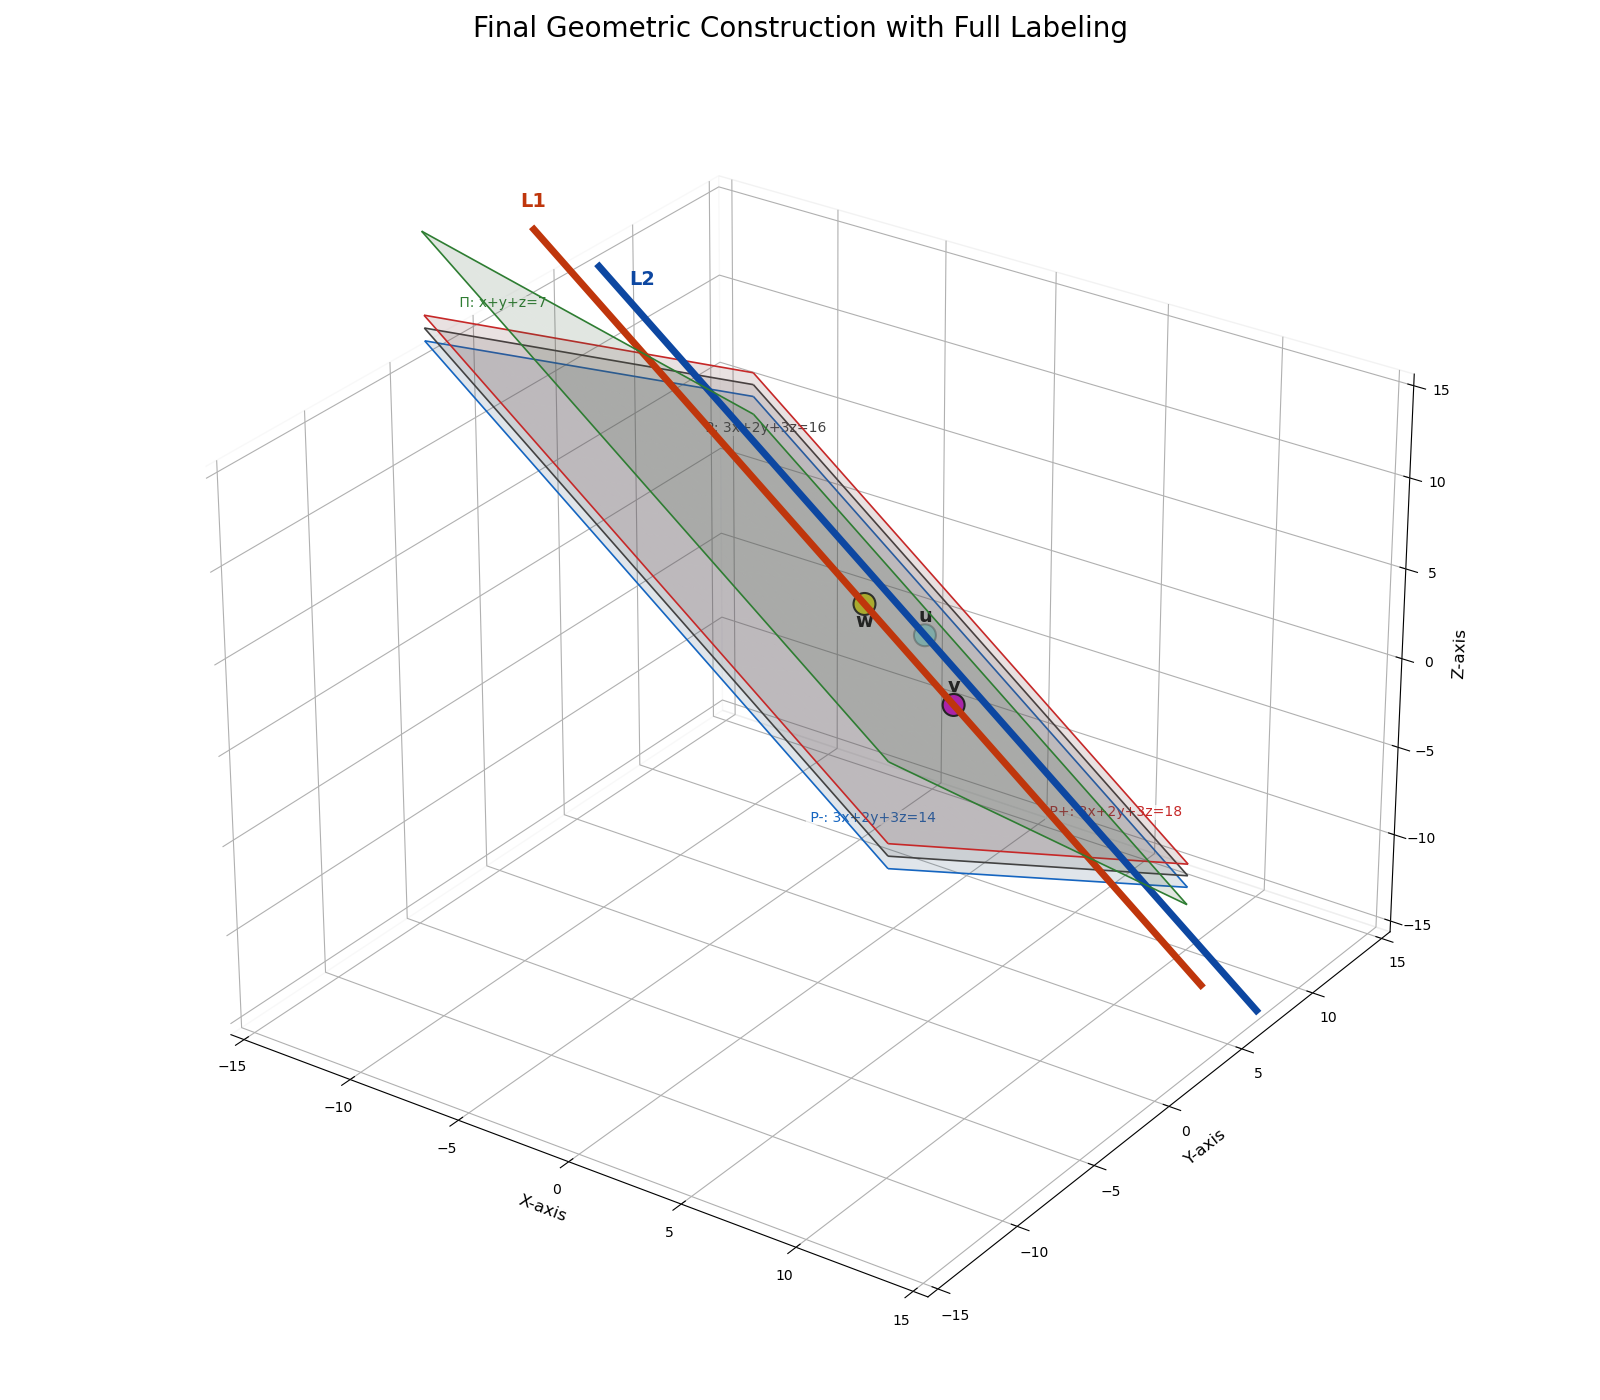
\includegraphics[width=0.9\columnwidth]{figs/fig5_.png} 
   \caption*{Fig: Representation of Planes and vectors}
  \label{Fig5}
\end{figure}

\end{document}
